\subsection{Conveyor Belt Test (CBT)}


\paragraph{Purpose and Focus of the Test}
The purpose of the Conveyor Belt Test is to assess the robot’s ability to manipulate moving objects which are placed on a conveyor belt. The test demands fast perception and manipulation skills in order to pick up objects from an operating conveyor belt.

\paragraph{Scenario Environment}
The same arena as for the Basic Manipulation Test is used (Figures 5.4 and 5.5). In case that the arena does not already include a conveyor belt (see Figure \ref{fig:conveyor_belt}), it will be added only for this particular test.
The OC may choose to use a rotating turntable instead of a linear conveyor belt in order to simplify the setup of the arena. The particular choice shall be announced before the tournament.
An area besides the conveyor belt is left free so that a robot can drive there and grasp the objects from the belt. The other sides might not be accessible, because the device is placed into a corner. 
The conveyor belt should have a wireless mechanism to turn it on. 

\begin{figure}
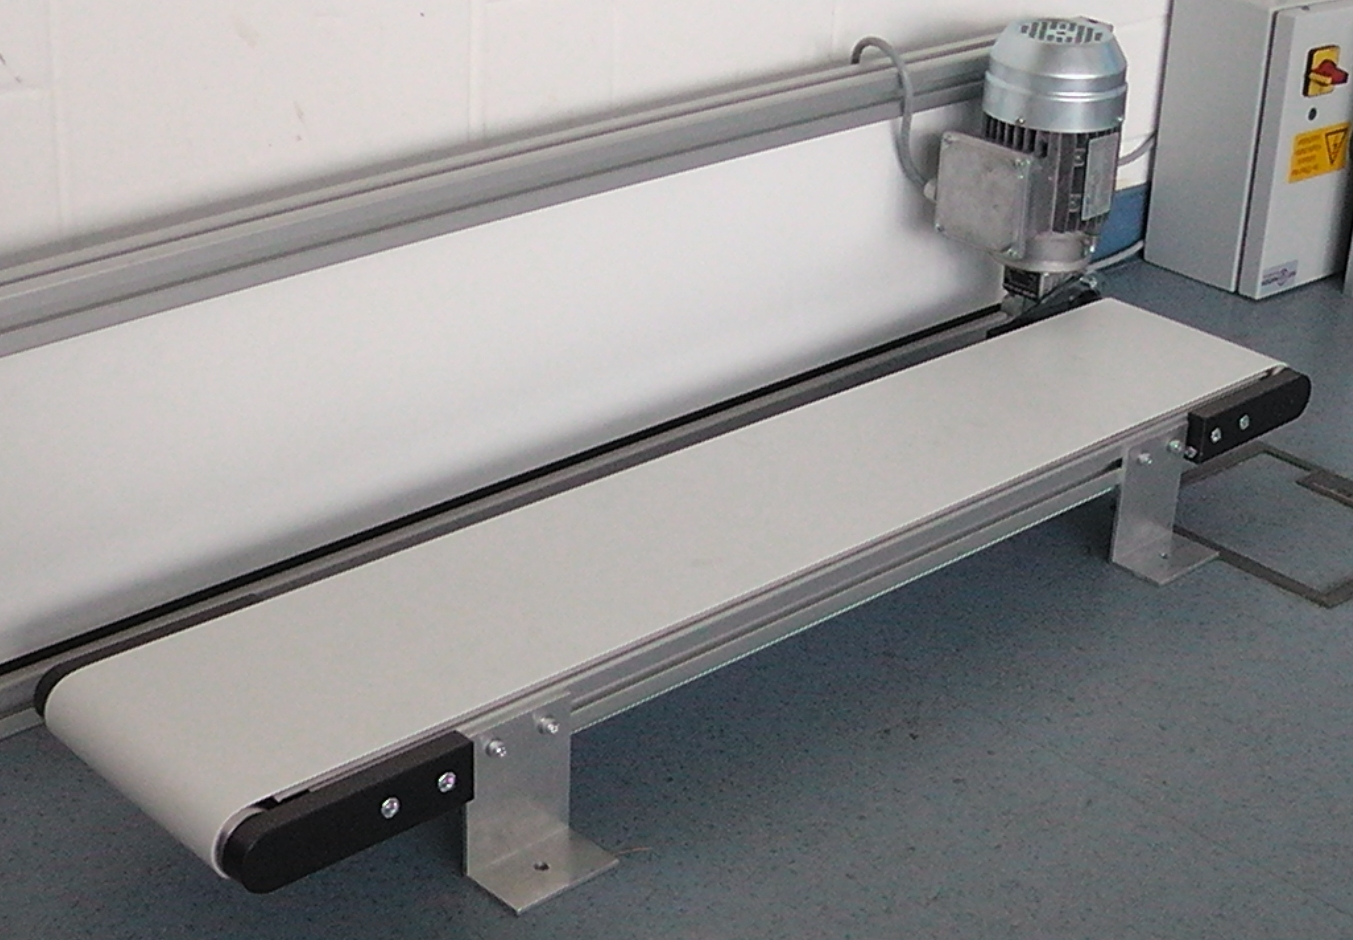
\includegraphics[width= \textwidth ]{../images/conveyor_belt.jpg}
\caption{Illustration of a conveyor belt used in the competition}
\label{fig:conveyor_belt}
\end{figure}


%\paragraph{Manipulation Objects}
%The same manipulation objects as for the Basic Manipulation Test are used. The team has to choose five objects out of the total object set (see Section 5.5.1). From those five objects, the TC is going to select three objects which will be placed on the conveyor belt. Beside these three objects there will be no other objects on the conveyor belt.

\paragraph{Task}
A single robot is used. The robot is placed by the team in some starting position outside of the arena. Initially the conveyor is switched off (i.e. the belt is not moving) and all objects are put on the belt with a distance between them determined by the TC. The task of the robot is to navigate to the location of the conveyor belt and to grasp all objects from the moving belt before they fall off at the other end of the belt. If a turntable is used, the objects can pass multiple times in front of the robot, until the maximum time for the run is over. The robot is supposed to place the grasped objects on the robot itself. The task is finished once the robot successfully grasped all objects or the foreseen time of the test has been exceeded. 
\par
There are two options to determine when to switch on the conveyor belt:
The robot starts it itself, using the wireless mechanism.
A team member can give a signal to the referees to switch on the conveyor belt.
\par
Teams can decide during the run to give the signal to the referees, e.g. when the robot failed to start it itself. 
\par
The task specification has the following structure:
\par
CBT \textless srv\_area\textgreater
\par
where ‘srv\_area’ is the location of the conveyor belt (e.g. T1)

%\subsection{Complexity Options}
%All Complexity Options from BMT apply.


%\subsubsection{Speed Complexity (pick one):}
%
%\begin{itemize}
%\item low speed (bonus factor = +0.0): The conveyor belt speed will be not more than 0.5 cm/s
%\item medium speed (bonus factor = +02):	The conveyor belt speed will be not more than 0.75 cm/s
%\item high speed (bonus factor = +0.4): The conveyor belt speed will be not more than 0.10 cm/s
%\end{itemize}



\paragraph{Rules}
The following rules have to be obeyed:

\begin{itemize}
\item The order in which the teams have to perform will be determined by a draw.
\item A team has a time period of 10 minutes to complete a run. The time is stopped when the robot has completed the task.
\item At the beginning of a team’s period, the team will get the task specification.
\item The objects are placed on the conveyor before the run starts, for low complexity by the team or for medium and high by a referee..
\item After the team’s robot starts, it must move inside the arena.
\item Either the robot itself starts the conveyor belt, or a team member can give a signal to the referees to switch on the conveyor belt..
\item The objects have to be grasped actively from the moving belt. The robot is not allowed e.g. to wait at the end with a particular basket and collect the falling objects from the end of the conveyor belt. Further, wiping the objects to the side is also not allowed.
\item A manipulation object counts as successfully grasped, if the robot has lifted the object and moved it outside of the area of the conveyor belt as specified in Section 5.5.3 point 2.
\item The team must leave the arena within a minute after completing the task.
\end{itemize}



%
%\subsection{Scoring}
%Points are awarded as follows:
%
%\begin{itemize}
%\item 200 points are awarded for successfully grasping an object from the conveyor belt 
%\item -150 points are given if an object dropped onto the ground, is placed not on the robot itself or dropped from the end of the conveyor..
%\item -100 points are given if the referees had to switch on the belt manually after signalled by a team member, while a working automatic wireless mechanism to switch it on was available.
%\item 50 points are awarded if the task has been fully achieved (when all objects placed on the belt are grasped).
%\end{itemize}
